\documentclass[tikz,border=7pt]{standalone}
\usepackage{amsmath,amssymb}
\usepackage[scaled]{helvet}
\renewcommand{\familydefault}{\sfdefault}
\usetikzlibrary{arrows.meta,backgrounds,calc,fit,positioning,shapes.geometric}
\definecolor{bpink}{HTML}{172033}
\definecolor{bpblue}{HTML}{2A78D6}
\definecolor{bporange}{HTML}{E56A32}
\definecolor{bpgreen}{HTML}{168A65}
\definecolor{bppurple}{HTML}{7A5CC7}
\definecolor{bpred}{HTML}{C94A4A}
\definecolor{bpmuted}{HTML}{667085}
\definecolor{bpgrid}{HTML}{D8DEE8}
\definecolor{bpsurface}{HTML}{F8FAFC}
\tikzset{
  var/.style={circle,draw=bpblue,fill=bpblue!10,line width=.9pt,minimum size=8mm,font=\small\bfseries,text=bpink},
  factor/.style={rectangle,rounded corners=1.5pt,draw=bporange,fill=bporange!14,line width=.9pt,minimum size=6.8mm,font=\small\bfseries,text=bpink},
  constraint/.style={rectangle,rounded corners=1.5pt,draw=bpred,fill=bpred!12,line width=.9pt,minimum size=6.8mm,font=\small\bfseries,text=bpink},
  edge/.style={draw=bpmuted!75,line width=.9pt},
  msgvf/.style={-{Latex[length=2.2mm]},draw=bpblue,line width=1.35pt},
  msgfv/.style={-{Latex[length=2.2mm]},draw=bporange,line width=1.35pt},
  label/.style={font=\scriptsize,text=bpmuted,align=center},
  title/.style={font=\bfseries\large,text=bpink},
  card/.style={draw=bpgrid,fill=bpsurface,rounded corners=7pt,line width=.7pt},
}

\begin{document}
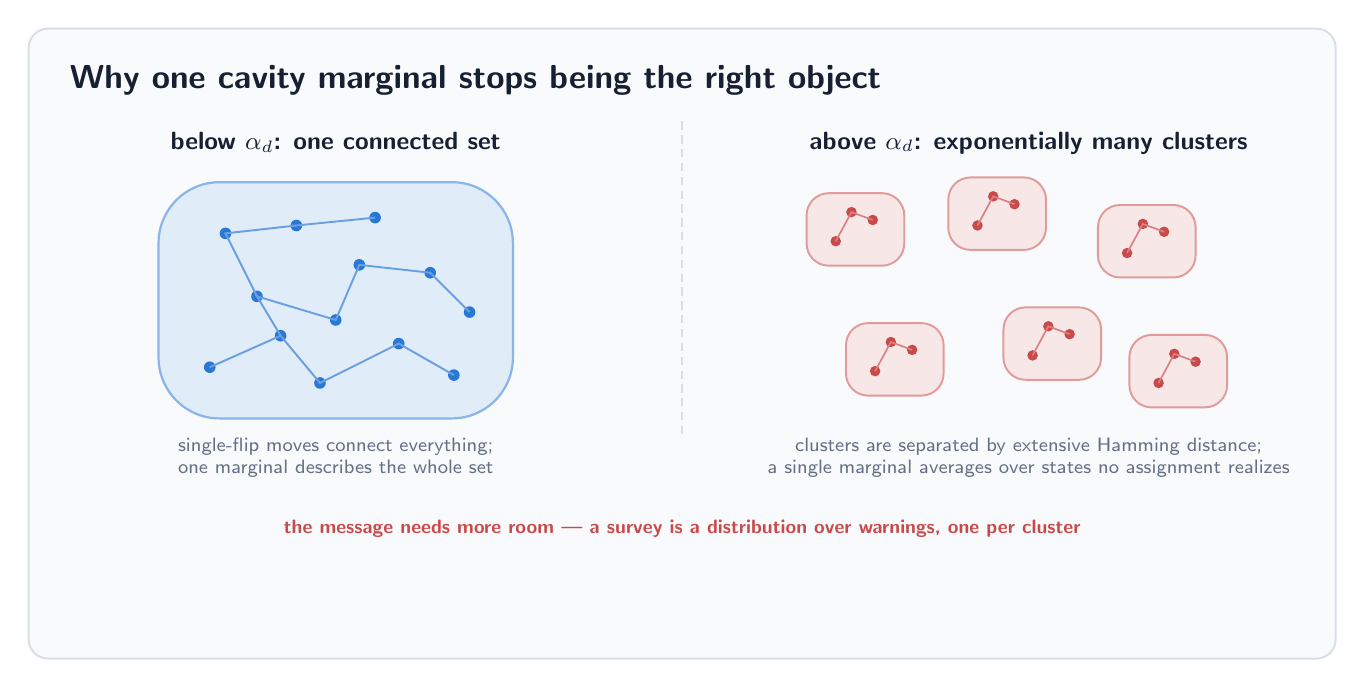
\begin{tikzpicture}[font=\sffamily]
  \node[card,minimum width=16.6cm,minimum height=8.0cm] at (7.5,2.7) {};
  \node[title,anchor=west] at (-.4,6.05) {Why one cavity marginal stops being the right object};

  % ---------------- replica-symmetric side ----------------
  \node[text=bpink,font=\small\bfseries] at (3.1,5.25) {below $\alpha_d$: one connected set};
  \begin{scope}[shift={(0,0)}]
    \fill[bpblue!14,rounded corners=22pt] (.85,1.75) rectangle (5.35,4.75);
    \draw[bpblue!55,rounded corners=22pt,line width=.8pt] (.85,1.75) rectangle (5.35,4.75);
    \foreach \x/\y in {1.5/2.4, 2.1/3.3, 1.7/4.1, 2.9/2.2, 3.1/3.0, 2.6/4.2, 3.9/2.7, 4.3/3.6, 3.6/4.3, 4.8/3.1, 4.6/2.3, 2.4/2.8, 3.4/3.7}
      \fill[bpblue] (\x,\y) circle (2.1pt);
    \draw[bpblue!70,line width=.7pt] (1.5,2.4)--(2.4,2.8)--(2.9,2.2)--(3.9,2.7)--(4.6,2.3);
    \draw[bpblue!70,line width=.7pt] (2.4,2.8)--(2.1,3.3)--(3.1,3.0)--(3.4,3.7)--(4.3,3.6)--(4.8,3.1);
    \draw[bpblue!70,line width=.7pt] (2.1,3.3)--(1.7,4.1)--(2.6,4.2)--(3.6,4.3);
  \end{scope}
  \node[label,align=center] at (3.1,1.25) {single-flip moves connect everything;\\one marginal describes the whole set};

  % ---------------- 1RSB side ----------------
  \node[text=bpink,font=\small\bfseries] at (11.9,5.25) {above $\alpha_d$: exponentially many clusters};
  \foreach \cx/\cy in {9.7/4.15, 11.5/4.35, 13.4/4.0, 10.2/2.5, 12.2/2.7, 13.8/2.35}{
    \fill[bpred!13,rounded corners=8pt] (\cx-.62,\cy-.46) rectangle (\cx+.62,\cy+.46);
    \draw[bpred!55,rounded corners=8pt,line width=.7pt] (\cx-.62,\cy-.46) rectangle (\cx+.62,\cy+.46);
    \fill[bpred] (\cx-.25,\cy-.15) circle (1.9pt);
    \fill[bpred] (\cx+.22,\cy+.12) circle (1.9pt);
    \fill[bpred] (\cx-.05,\cy+.22) circle (1.9pt);
    \draw[bpred!70,line width=.6pt] (\cx-.25,\cy-.15)--(\cx-.05,\cy+.22)--(\cx+.22,\cy+.12);
  }
  \node[label,align=center] at (11.9,1.25) {clusters are separated by extensive Hamming distance;\\a single marginal averages over states no assignment realizes};

  % divider + verdict
  \draw[bpgrid,line width=.9pt,densely dashed] (7.5,1.55) -- (7.5,5.55);
  \node[text=bpred,font=\scriptsize\bfseries,align=center] at (7.5,.35)
    {the message needs more room — a survey is a distribution over warnings, one per cluster};
\end{tikzpicture}
\end{document}
